% !TeX spellcheck = ru_RU
% !TEX root = mainrus.tex

\section{Реализация и эксперименты}

\begin{figure*}[t]
\begin{verbnobox}[\fontsize{10pt}{10pt}\selectfont]
ordered main_group (
  Label "Type" describes TextEdit "Any" {width=200}
  Label "Owner" describes TextEdit "Anyone" {width=200}
  Label "Has the words" describes TextEdit "Enter words found in the file" {
   width = 400
  }
  Label "Item name" describes
    TextEdit "Enter a term that matches part of the file name" {
      width = 400
    }
  (Label "Location" describes
    (TextEdit "Anywhere" { width = 200 }) dominates
    ordered location_checkboxes (
      Label "In trash"  describes CheckBox in_trash_checkbox
      Label "Starred"   describes CheckBox starred_checkbox
      Label "Encrypted" describes CheckBox encrypted
    )
  )
  Label "Date modified" describes  TextEdit "Any time" {width=200}
  Label "Approvals" describes
    ordered approvals_checkboxes (
      Label "Awaiting my approval" describes CheckBox awaiting_checkbox
      Label "Requested by me" describes CheckBox requestred_checkbox
  )
  Label "Shared to" describes
    TextEdit "Enter a name or email address..." {width=400}
  Label "Follow-ups" describes TextEdit "---" {width=200, height=35}
)
Button "Search" approves^ main_group
Button "Reset" cancels^ main_group
\end{verbnobox}
\caption{Описание структура диалога поиска из сервиса Google Drive}
\label{gd_structure}
\end{figure*}

\begin{figure*}[t]
    \begin{subfigure}[t]{.45\textwidth}
        \vspace{-15em}
        \begin{minipage}{4cm}
        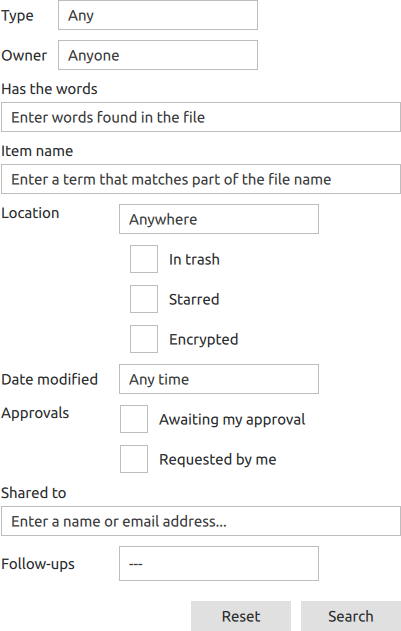
\includegraphics[scale=0.5]{../google-drive-search-setting-output2.png}
        \end{minipage}
        \caption{Если метка описывает \enquote{слишком длинный} элемент управления, то располагать их вертикально}
    \end{subfigure}\hspace{1cm}
    \begin{subfigure}[t]{.45\textwidth}
      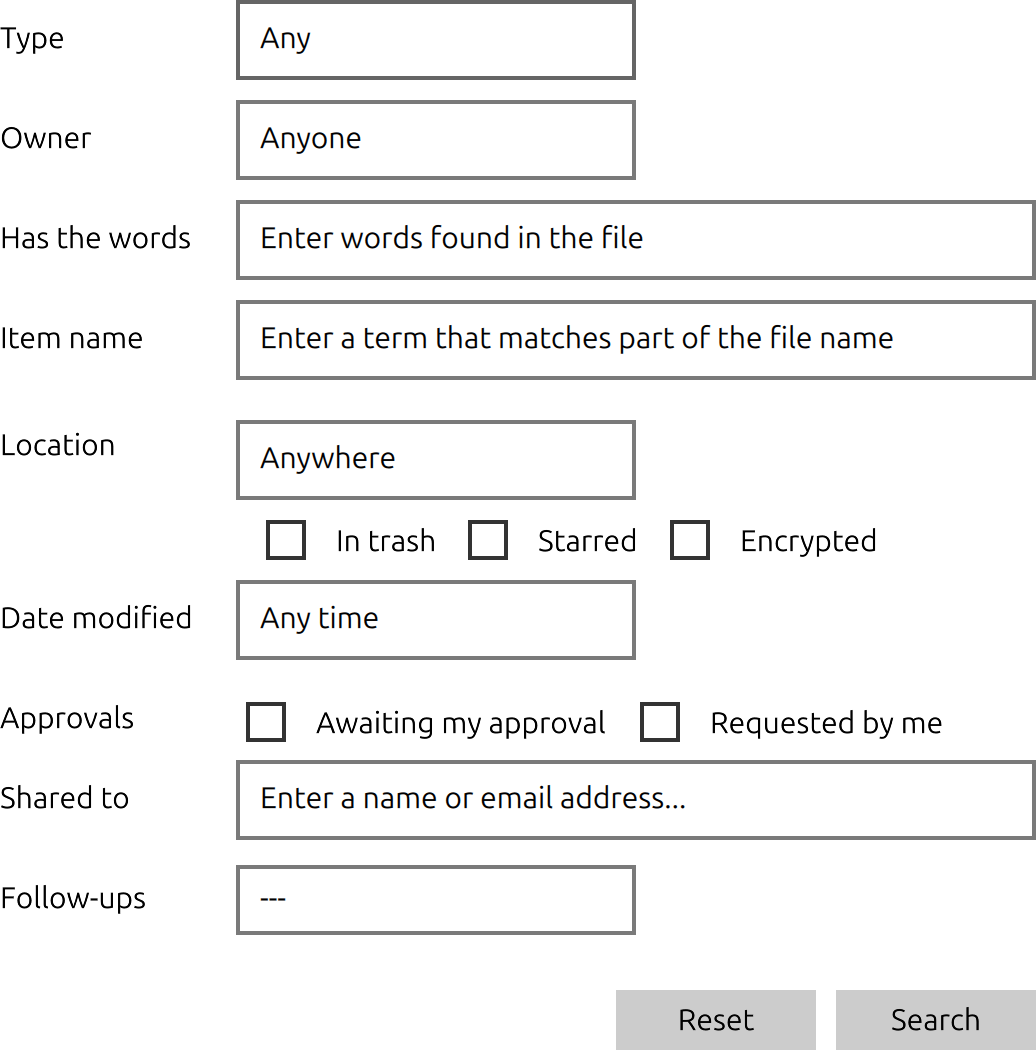
\includegraphics[scale=0.5]{../google-drive-search-setting-output3.png}
      %\vskip17.5mm
      \caption{То же самое, но константа для свойства  \enquote{слишком длинный} уменьшена}
    \end{subfigure}
    \caption{Синтезированные расположения элементов для диалога из Google Drive}
    \label{fig:QMLtwoGuidelines}
\end{figure*}



Прототип синтезатора реализован как клиент-серверное приложение\footnote{Прототип доступен по ссылке:
\url{https://se.math.spbu.ru/projects/genui} (проверено: \DTMDate{2024-08-26})}.
Со стороны клиента мы используем \textsc{HTML5} и \JavaScript{} для взаимодействия с сервером\footnote{\textcolor{red}{Реализация от Дениса сейчас не использует \JSOO.} Вернуться к этому }.
На сервере исполняется \OCaml приложение, оснащённое \OCanren{} и \Zthree{}.

%The prototype of our synthesizer is developed as a \mbox{client}/server application using web technologies\footnote{The implementation is available online
%for review: \url{https://genui.utbot.org}, username: ``public-user'', password: ``1jWMz2oWWmQW40hHSPZb'', no quotes.
%%In case it doesn't work try \url{https://se.math.spbu.ru/genui}.
%Generated design will be shown below specification field.}.
%On the client side we use \textsc{HTML5} for rendering and \OCaml
%compiled to \textsc{JavaScript} via \JSOO~\cite{JSOO} for a client-server interaction. The server side is a native \OCaml application equipped with \OCanren and \Zthree.

Чтобы облегчить пользователю представление структуры GUI и гайдлайна, мы разработали два текстовых предметно-ориентированных языка.
В реализации выразительность языка гайдлайнов   расширена: мы разрешаем в правилах использовать пользовательские ограничения, присутствуют конструкции для задания табличных расположений, и т.п. Ни одно из расширений существенно не изменяет подход, описанный в предыдущих главах, и все расширения могут быть учтены.
Мы также параметризуем систему набором констант, которые определяют свойства окружения (например, размер холста, где мы располагаем элементы управления).
Пример описания структуры для диалогового окна настроек поиска сервиса Google Drive представлена на рис.~\ref{gd_structure}.
Текстовое описание гайдлайна слишком длинное, чтобы представить его здесь.

%In order to provide end-users a way to represent GUI structures and guidelines we developed two textual DSLs. In addition in our implementation
%the expressivity of guidelines description was a little bit extended~--- for example, we actually allow the rules to be equipped with custom constraints, there are
%some extra constructs to express the guidelines for table-like layouts, etc. None of these extensions compromise the approach we
%described in the previous sections and all of them can rather easily be taken into account. We also parameterized our system with
%a set of constants which describe the common properties of the environment (for example, the size of the pane to place the synthesized layout in).
%An example of structure description for Google Drive search settings dialog is shown in Fig.~\ref{gd_structure}.
%The textual representation of guidelines, however, is too lengthy to show.


\begin{comment}
The flowchart of server-side application architecture is shown in Fig.~\ref{server-flowchart}. Dotted blocks denote the input data (structure,
guideline and environment descriptions), blocks with solid thin borders~--- \OCaml non-relational components, blocks with solid thick borders~---
relational components written in \OCanren. Thin arrows show the data transfer between components, and the thick one~--- the execution
of generated from inputs relational program. By ``run$^*$'' we denote the execution of relational components which return all the answers for the problem
they solve. The last two steps (integer linear inequations generation and \Zthree execution) are performed for each synthesized hypercube.

\begin{figure}[h]
%  \centering
  \includegraphics[scale=0.5]{server-flowchart.eps}   % if it fails to compile install 'texlive-font-utils'
  \caption{The architecture of server-side application}
  \label{server-flowchart}
\end{figure}
\end{comment}

\begin{comment}
\begin{figure*}
  \begin{tabular}{m{7.5cm}|m{10.5cm}}
    \begin{lstlisting}[basicstyle=\small]
| Descr (l, cb), Type (cb, CheckBox)
  => Hor (cb, l)

| Ord (x, y) => Vert (x, y), Halign (x, y)

| Sub (x, y) => Vert (x, y), Indent (x, y)

\end{lstlisting} & \multirow{3}{*}{
\begin{tabular}{c}
	\parbox{9cm}{There are no such explicit rules in the guideline, but these basic cases implicitly follow from the others.}
\end{tabular}}\\
\hline
\begin{lstlisting}[basicstyle=\small]
| Descr (X, Y), not (Type (Y, Checkbox)),
  width (Y) <= K
  => Hor (X, Y)
\end{lstlisting} & \multirow{2}{*}{
\begin{tabular}{c}
	{ \parbox{9.5cm}{
					\vspace{-1em}
If an input box is long, and the horizontal space is limited, place the label above the box. Otherwise, always put the label and the box on the same line.
	}}\\
  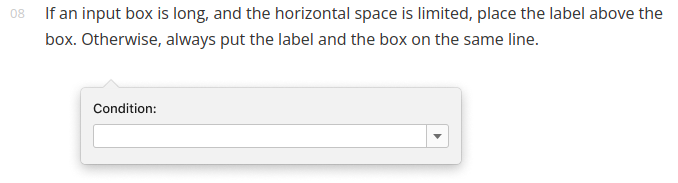
\includegraphics[scale=0.3]{jbg-08.png} \\
%  \includegraphics[scale=0.3]{jbg-08-new.png} \\
  {\parbox{9.5cm}{\textit{By the second rule variable $X$ is a label with text ``Condition'' and variable $Y$ is a drop-down list.}}}
\end{tabular}}\\
\begin{lstlisting}[basicstyle=\small]
| Descr (X, Y), not (Type (Y, Checkbox)),
  width (Y) > K
  => Vert (X, Y), Halign (X, Y)
\end{lstlisting} & \\ \\
\hline
\begin{lstlisting}[basicstyle=\small]
| Ord (v1, v2),
  Comp (v1, c1), not (Type (c1, CheckBox)),
  Comp (v2, c2), not (Type (c2, CheckBox)),
  Descr (l1, c1), Descr (l2, c2),
  width c1 $\leqslant\!$ 100, width c2 $\leqslant\!$ 100
  => (
  | width l1 $\!\geqslant\!$ width l2, width l1 $\leqslant\!$ width l2 $\cdot$ 2
  | width l1 $\!<\!$ width l2, width l2 $\leqslant\!$ width l1 $\cdot$ 2
    => Halign (c1, c2))
\end{lstlisting} &
\begin{tabular}{c}
{\parbox{9.5cm}{
%		\vspace{-4em}
	By default, put input controls with labels of similar length on different lines and align their input boxes on the left side.
}}\\
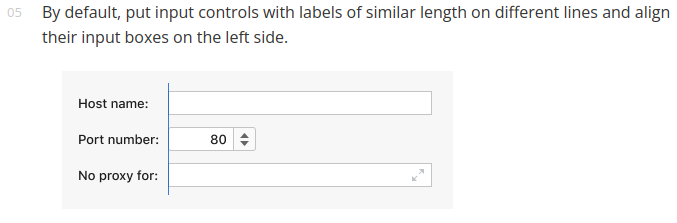
\includegraphics[scale=0.3]{jbg-05.png} \\
%\includegraphics[scale=0.2]{jbg-05-new.png} \\
{\parbox{9.5cm}{\textit{The rule applied twice. In the first case virtual control $C$ contains the top textbox $Y$ and virtual control $C^\prime$ contains the middle textbox $Y^\prime$. The textbox $Y$ is described by the top label $X$ and the textbox $Y^\prime$ is described by the middle label $X^\prime$. The second case is similar for middle and bottom controls.}}}
\end{tabular}
\\
\\
\hline
\begin{lstlisting}[basicstyle=\small]
| Ord (v1, mid),
  Ord (mid, v2),
  Comp (v1, c1), not (Type (c1, CheckBox)),
  Comp (v2, c2), not (Type (c2, CheckBox)),
  Descr (l1, c1), Descr (l2, c2),
  width c1 $\leqslant\!$ 100, width c2 $\leqslant\!$ 100
  => (
  | width l1 $\!\geqslant\!$ width l2, width l1 $\leqslant\!$ width l2 $\cdot$ 2
  | width l1 $\!<\!$ width l2, width l2 $\leqslant\!$ width l1 $\cdot$ 2
    => Halign (c1, c2))
\end{lstlisting} &
\begin{tabular}{c}
{\parbox{9.5cm}{
%		\vspace{-4em}
	If there are two input controls with labels of similar length that are separated from each other by a single control, align their input boxes on the left side.
}}\\
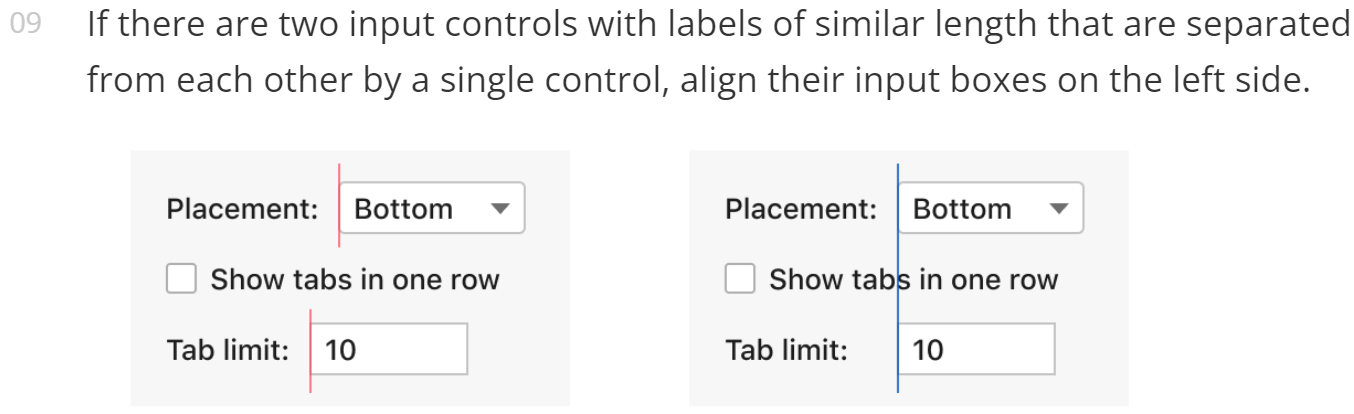
\includegraphics[scale=0.3]{jbg-09.png} \\
%\includegraphics[scale=0.4]{jbg-09-new.png} \\
{\parbox{9.5cm}{\textit{By the rule virtual control $C$ contains the top textbox $Y$ and virtual control $C^{\prime}$ contains the bottom textbox $Y^\prime$. There is a virtual control $Y^{\prime\prime}$ containing the checkbox between them. Labels $X$ and $X^\prime$ describe textboxes $Y$ and $Y^\prime$.}}}
\end{tabular}
  \end{tabular}
  \caption{Examples of GUI guidelines specification (based on informal JetBrains guidelines rules 05, 08 and 09)}
  \label{guidelines-example}
\end{figure*}
\end{comment}

%\subsection{Client Side}
%A web page is essentially a text area for the user input of structure information in the syntax similar to that in Fig.~\ref{fig:evaluation},
%and a space for rendering results. The client-server interaction runs in several phases. The client sends structure information to the server and receives possibly many layouts. After that it sends the %layouts to the server one by one and receives the exact coordinates of the UI elements in the structure. The layouts which were successfully evaluated with \Zthree are being rendered in the end.

%\subsection{Server Side}
%The server side is implemented in \OCaml with assistance of \OCanren\footnote{
%\href{https://github.com/PLTools/OCanren}{https://github.com/PLTools/OCanren}
%\url{https://github.com/PLTools/OCanren}
%}~\cite{Zthree}, \noCanren\footnote{\url{https://github.com/Lozov-Petr/noCanren}}~\cite{lozov2017typed}
% and \Zthree~\cite{Zthree}. It could be separated into two parts: synthesis of a layout and evaluation of absolute coordinates.

%The synthesis of a layout is implemented mostly in functional style with assistance of \noCanren, which translates a dialect of \textsc{ML} to \OCanren. The exception is a
%confirmation check (described in Section~\ref{sec:synthesizing}) which is easier to implement in relational style because it applies non-deterministically many guideline rules.
%Encoding of the guideline rules themselves in \OCanren is error-prone because of inversion requirement. We implemented an embedded DSL for \OCaml for these guidelines
%which performs an inversion at compile time.

%We could name two drawbacks in our current implementation.  For now we have a limited amount of identifiers for UI elements (named by letters from A to J on
%Figure \ref{fig:evaluation}) which allows to represent our binary hypercube finitely, but
%reduces the expressivity of input structure definition. In future it shall be easily fixed because all possible structure definitions have a finite number
%of elements. Another drawback of our binary hypercube is an ability to encode nonsensical layouts (for example, one element subordinates another and vice versa).
%Right now these layouts are filtered out during the generation of absolute coordinates, but ideally we want them to be non-representable using type definitions of our synthesizer.

%The second part of server implementation is the calculation of absolute coordinates with assistance from \Zthree. This stage filters out problematical layouts and performs much
%faster than our relational synthesis. But we linked \OCaml and \Zthree to a single executable anyway  to avoid paying any costs  for inter process communication.

Для оценки нашего прототипа на промышленных примерах мы также реализовали отображение элементов управления с помощью Qt/QML.
На рис.~\ref{fig:QMLtwoGuidelines} можно увидеть два расположения структуры диалогового окна Google Drive, синтезированного
с учетом двух немного различных версий гайдлайна от JetBrains~\cite{JBG}, нарисованные с помощью  QtQuick Controls\footnote{\url{https://doc.qt.io/qt-5/qtquick-controls2-qmlmodule.html}} и темы оформления Material Design.
Гайдлайн регламентирует, что \enquote{слишком длинный} текст должен располагаться под меткой.
На правом расположении константа, регламентирующая свойство \enquote{слишком длинный} была уменьшена. Синтез занял примерно 5 секунд.

%The guideline says that if a text edit is ``too long'', one has to put it below the label.
%On the bottom layout the
%factor describing the informal notion of ``being too long'' was increased. The synthesis of each layout took 5 seconds.

Некоторые другие примеры можно найти на рис.~\ref{fig:evaluation}.


%To evaluate our prototype in the context of the real world GUI framework we implemented a renderer based on Qt/QML. On Fig.~\ref{fig:QMLtwoGuidelines} you can see two layouts of the
%Google Drive search settings dialog structure rendered  w.r.t. two slightly different versions of JetBrains GUI guidelines~\cite{JBG} using QtQuick Controls\footnote{\url{https://doc.qt.io/qt-5/qtquick-controls2-qmlmodule.html}} and Material Design theme. The guideline says that if a text edit is ``too long'', one has to put it below the label.
%On the bottom layout the
%factor describing the informal notion of ``being too long'' was increased. The synthesis of each layout took 5 seconds.
%
%A few more examples are shown in Fig.~\ref{fig:evaluation}.



\begin{figure*}
    \begin{tabular}{m{95mm}m{5cm}}
      \begin{lstlisting}[basicstyle=\small]
  ordered (
    Label "Short label"
       describes TextEdit "Text 1"
    Label "Loooooong label"
       describes TextEdit "Text 2"
  )
      \end{lstlisting} &
      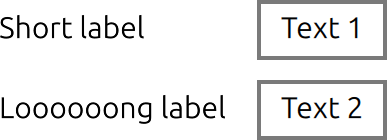
\includegraphics[scale=0.5]{../Example1-Qt-QML.png} \\
      \hline\\
      \begin{lstlisting}[basicstyle=\small]
  ordered (
    Label "Looooong label"
        describes TextEdit "Text 1"
    Label "Medium label"
        describes TextEdit "Text 2"
    Label "Short"
        describes TextEdit "Text 3"
  )
      \end{lstlisting} &
      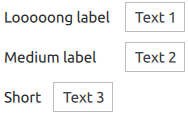
\includegraphics[scale=0.5]{../Example2-Qt-QML.png} \\
      \hline
      \begin{lstlisting}[basicstyle=\small]
  ordered (
    Label "Short label"
        describes TextEdit "Text 1"
    Label "Check box label"
        describes CheckBox _
    Label "Looooong label"
        describes TextEdit "Text 2"
  )
      \end{lstlisting} &
      \vspace{1em}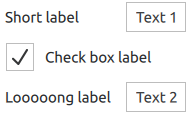
\includegraphics[scale=0.5]{../Example4-Qt-QML.png} \\
      \hline\\
      \begin{lstlisting}[basicstyle=\small]
  ordered (
    Label "L 1"     describes CheckBox _
    Label "Lab 2"   describes CheckBox _
    Label "Label 3" describes CheckBox _
    Label "Label 4" describes CheckBox _
    Label "L 5"     describes CheckBox _
    Label "Lab 6"   describes CheckBox _
  )
      \end{lstlisting} &
      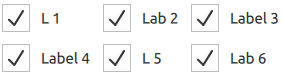
\includegraphics[scale=0.5]{../Example5-Qt-QML.png} \\
    \end{tabular}
    \caption{Примеры структур (слева) и синтезированных расположений (справа)\\
      с учётом гайдлайна от  JetBrains}
    \label{fig:evaluation}
  \end{figure*}
